\documentclass[12pt,a4paper]{article}
\usepackage[T1]{fontenc}
\usepackage[utf8]{inputenc}
\usepackage[english]{babel}
\usepackage{array, booktabs}
\usepackage[table]{xcolor}
\setlength{\aboverulesep}{0pt}
\setlength{\belowrulesep}{0pt}
\newcommand\VRule[1][\arrayrulewidth]{\vrule width #1}
\usepackage{graphicx}
\graphicspath{ {./plots/} }
\usepackage{enumitem}
\usepackage{tabularray}
\usepackage{siunitx}    
\usepackage{float}
\usepackage[top=2cm, bottom=2cm, left=2.5cm, right=2.5cm]{geometry}
\usepackage{tabularray}
\usepackage{amsmath,amsfonts,amssymb}

\title{\textbf{Coursework for Algorithms for Data Analysis and Data Mining
	(I+II)}}
\author{
	\begin{tabular}{ccc}
		\textbf{Hasan Mahmood}, & 804251, & s804251@sggw.edu.pl \\
		\textbf{Jan Pokraśniewicz}, & 227738, & s227738@sggw.edu.pl \\
		\textbf{Maciej Lemeański}, & 227781, & s227781@sggw.edu.pl \\
		\textbf{Tomasz Żołądek}, & 230998, & s230998@sggw.edu.pl \\
	\end{tabular}
}
\date{08.05.2026}

\begin{document}
	\maketitle
	\part*{A. Data Analysis and Regression}
	\section{Logistic Regression}
	\indent \indent Data provided for analysis with logistic regression was placed in a table below.
	\begin{table}[htbp]
		\centering
		\caption{Numbers of hours on programming and final result.}
		\label{label}
		\begin{tabular}{!{\VRule[1.5pt]} c | *{10}{c} !{\VRule[1.5pt]}}
			\specialrule{1.5pt}{0pt}{0pt}
			Hours & 25 & 35 & 40 & 50 & 55 & 60 & 70 & 89 & 92 & 100  \\\hline
			Result & 0 & 0 & 0 & 1 & 0 & 1 & 1 & 1 & 1 & 1  
			\\\specialrule{1.5pt}{0pt}{0pt}
		\end{tabular}
	\end{table}
	\begin{enumerate}[label=\alph*)]
		\item For this exercise we used code from file "ZadA1a.R". \newline Summarizing the logistic regression for provided data set we receive following parameters:
		\newline
		\begin{center}
			\begin{tabular}{!{\VRule[1.5pt]} c !{\VRule[1.2pt]} *{3}{c|} c !{\VRule[1.5pt]}}
				\specialrule{1.5pt}{0pt}{0pt}
				Variable & Estimate  & Std. Error & z value & $p$-value
				\\\specialrule{1.2pt}{0pt}{0pt}
				Intercept & -10.8360 & 8.3232 & -1.302 & 0.193 \\\hline
				x & 0.2091 & 0.1576 & 1.327 & 0.185
				\\\specialrule{1.5pt}{0pt}{0pt}
			\end{tabular}
		\end{center}
		As we may see, basing on data from table 2, the z values for both variables are rather high what is proven by $p$-value being higher than 0.1 what can be considered as quite large. It is indeed result of low amount of data - 10 records equivalent to 9 degrees of freedom. This means that significance of our model is low thus statistically it is not important. Nevertheless, we may conclude that direction of dependence between hours of programming and final result is positive.
		\newline We may also plot the graph below and find out that midpoint value is 51.83.
		\newline
		
\includegraphics[scale=0.5]{plot1Aa}
		\item For this exercise we used code from file "ZadA1b.R". 
		\newline Summarizing the logistic regression for provided data set, excluding point (100, 1), we receive following parameters:
		\begin{center}
			\begin{tabular}{!{\VRule[1.5pt]} c !{\VRule[1.2pt]} *{3}{c|} c !{\VRule[1.5pt]}}
				\specialrule{1.5pt}{0pt}{0pt}
				Variable & Estimate  & Std. Error & z value & $p$-value
				\\\specialrule{1.2pt}{0pt}{0pt}
				Intercept & -10.8360 & 8.3232 & -1.302 & 0.193 \\\hline
				x & 0.2091 & 0.1576 & 1.327 & 0.185
				\\\specialrule{1.5pt}{0pt}{0pt}
			\end{tabular}
		\end{center}
		As we may see value of all parameters is the same as from the a) sub-point. 
		\newline
		
\includegraphics[scale=0.5]{plot1Ab}
		\\ Moreover, the graph is also the same including midpoint value. Thus, we may conclude that removing point (100, 1) does not influence this model. We may suppose that it influenced by almost perfect correspondence of coordinates of this point with proposed model.
		\item For this exercise we used code from file "ZadA1c.R". 
		\newline Summarizing the logistic regression for data set from sub-point a, including new point (115, 1), we receive following parameters:
		\begin{center}
			\begin{tabular}{!{\VRule[1.5pt]} c !{\VRule[1.2pt]} *{3}{c|} c !{\VRule[1.5pt]}}
				\specialrule{1.5pt}{0pt}{0pt}
				Variable & Estimate  & Std. Error & z value & $p$-value
				\\\specialrule{1.2pt}{0pt}{0pt}
				Intercept & -10.8360 & 8.3232 & -1.302 & 0.193 \\\hline
				x & 0.2091 & 0.1576 & 1.327 & 0.185
				\\\specialrule{1.5pt}{0pt}{0pt}
			\end{tabular}
		\end{center}
		As we may see value of all parameters is the same as from the a) and b) sub-points. 
		\newline
		
\includegraphics[scale=0.5]{plot1Ac}
		Moreover, the graph is also the same. This is not surprising as it confirms hypothesis from sub-point b) that when coordinates is almost perfectly corresponding with our model. This we may conclude, that the model would only change if value on y axis were 0 which we would then consider as outlier. But ones placed on x axis to the right and keeping y=1 does not affect model.
		\item To sum up all above we may propose advantages and disadvantages
		\begin{center}
			\renewcommand{\arraystretch}{1.5} 
			\begin{tabular}{|p{0.45\textwidth}|p{0.45\textwidth}|}
				\hline
				\rowcolor{gray!20} 
				\textbf{Advantages} & \textbf{Disadvantages} \\
				\hline
				\cellcolor{green!10} Simple algorithm & \cellcolor{red!10} Very sensitive to outliers \\
				\hline
			\end{tabular}
		\end{center}
	\end{enumerate}
	
	\section{Nonlinear Least-Squares}
	\indent \indent Data provided for analysis with logistic regression was placed in a table below.
	\begin{table}[htbp]
		\centering
		\caption{Measured data points.}
		\label{label}
		\begin{tabular}{!{\VRule[1.5pt]} c | *{7}{c} !{\VRule[1.5pt]}}
			\specialrule{1.5pt}{0pt}{0pt}
			x & 0.1 & 0.5 & 1 & 1.5 & 2.05 & 2.5 & 3  \\\hline
			y & 0.23 & 0.65 & 0.9 & 0.8 & 0.7 & 0.6 & 0.5  
			\\\specialrule{1.5pt}{0pt}{0pt}
		\end{tabular}
	\end{table}
	And models provided for analysis are presented below:
	\begin{center}
		\begin{equation}
			y = 
			\begin{cases}
				f1(x) = \frac{ax}{b+cx^{2}} \\
				f2(x) = axe^{-bx + c} \\
				f3(x) = a + bx + cx^{2} + dx^{3}
			\end{cases}
		\end{equation}
	\end{center}
	\begin{enumerate}[label=\alph*)]
		\item For this exercise we will be using code from file 'ZadA2a.R'
		\newline Unfortunately, first 2 models cannot be fitted, at least with Nonlinear Least-Squares implemented in R as nls() function, as they lead to singular matrices. Thus we have to change their form to avoid this problem by simplifying them.
		\begin{center}
			\begin{equation}
				y = 
				\begin{cases}
					f1(x) = \frac{ax}{b+cx^{2}} = 
							\frac{ax}{\frac{1}{b}(1+\frac{c}{b}x^{2})} = \frac{\frac{a}{b}x}{1+\frac{c}{b}x^{2}} =
							\left\{
								\begin{array}{ll}
									d = \frac{a}{b} \\
									e = \frac{c}{b}
								\end{array}
							\right\} =	
							\frac{dx}{1+ex^{2}} \\
					f2(x) = axe^{-bx + c} =
							ae^{c}xe^{-bx} =
							\left\{
							\begin{array}{ll}
								d =  ae^{c}
							\end{array}
							\right\} =
							dxe^{-bx}
				\end{cases}
			\end{equation}
		\end{center}
		As the third model does not need any changes we finish with following forms of models:
		\begin{center}
			\begin{equation}
				y = 
				\begin{cases}
					f1(x) = \frac{dx}{1+ex^{2}} \\
					f2(x) = dxe^{-bx} \\
					f3(x) = a + bx + cx^{2} + dx^{3}
				\end{cases}
			\end{equation}
		\end{center}
		and graph presented below.
		\newline
		
\includegraphics[scale=0.5]{plotA2a}
		\item For this exercise we will be using the same code.
		\newline The errors of each model are presented in a table below:
		\begin{center}
			\begin{tblr}{
					cell{2}{4} = {r},
					cell{3}{4} = {r},
					cell{4}{4} = {r},
					vline{1-2,5} = {1}{},
					vline{1,5} = {2-4}{},
					vline{2} = {2-4}{gray!80},
					hline{1-2,5} = {-}{},
				}
				Model & RSE   & RMSE  & Difference \\
				f1(x) & 0.037 & 0.032 & 0.005      \\
				f2(x) & 0.037 & 0.031 & 0.006      \\
				f3(x) & 0.041 & 0.027 & 0.014      
			\end{tblr}
		\end{center}
		As we may see, the difference between RSE and RMSE errors is small for f1 and f2, especially compering them to the one for f3 which is larger by an order in magnitude. Nevertheless, it should not be surprising as f1 and f2 models bases on 2 parameters, as we decreased amount by 1 parameter to simplify equation, when f3 bases on 4! It is worth noting that the larger the difference is, the more model tends to over-fit. Moreover, if we had not simplified the models f1 and f2 the results might have been different! However, basing on data from the table above we should reject the third model because of too large tendency to over-fit. To choose the best one between f1 and f2, considering similar, low difference, we should choose one with lowest RMSE, thus the f2.
		
		\item For this exercise we will be using code from file 'ZadA2c.R' and the same models as at sub-point a) and b) but the data set is extended with additional point (4, 0.25). As a result, new graph has been plotted:
		\newline 
		
\includegraphics[scale=0.5]{plotA2c}
		\newline
		and a new table of errors has been created:
		\begin{center}
			\begin{tblr}{
					cell{2}{4} = {r},
					cell{3}{4} = {r},
					cell{4}{4} = {r},
					vline{1-2,5} = {1}{},
					vline{1,5} = {2-4}{},
					vline{2} = {2-4}{gray!80},
					hline{1-2,5} = {-}{},
				}
				Model & RSE   & RMSE  & Difference \\
				f1(x) & 0.048 & 0.041 & 0.007      \\
				f2(x) & 0.054 & 0.046 & 0.008      \\
				f3(x) & 0.079 & 0.056 & 0.023      
			\end{tblr}
		\end{center}
		As we may see, the graph and table for data set extended by point (4, 0.25) differs a lot to the ones without it. Both on the graph and in the table (larger difference) we can see how f3 'explodes' between the last points when the step on x axis is larger what is an another proof for thesis that f3 is over-fitting model. Moreover, we can see that difference between errors for f1 and f2 models did not change a lot. Thus, we can say that adding new point did not significantly increase instability. However, there is noticeable difference in errors between f1 and f2 what implies that positively f1 better fits the extended data set.
		\item To sum up, we can avoid over-fitting by using more simply thus ones with less parameters and lower degree of polynomial. Therefore, without doubt we can say that model f3 is too complex which leads to over-fitting which mean they have too much parameters. Because we have abbreviated the f1 and f2 model we must say that not only do original ones have too much parameters, thus they may over-fit, but finding the best fit with Nonlinear Least-Squares is impossible as, for such an amount of parameters, we cannot find one, most optimal solution.
	\end{enumerate}
	
	\clearpage
	\setcounter{section}{0}
	\part*{B. kNN Regression Analysis}
	\section{Summary of the sggw.b data}
		
		Here we used code from ZadB.R file.
		We will provide statistical analysis for the data. We have 10 explanatory features and one target feature - the price of the house. In the explanatory features (X-features) we have the Area, the numbers of Bathrooms, Bedrooms etc, and binary features telling us if there is metro in close proximity, is the place furnished, or is it a popular area.
		\\
		
		\begin{table}[H]
			\centering
			\begin{tblr}[         %% tabularray outer open
				]                     %% tabularray outer close
				{                     %% tabularray inner open
					colspec={Q[]Q[]Q[]Q[]Q[]},
					hline{2}={1-5}{solid, black, 0.05em},
					hline{1}={1-5}{solid, black, 0.08em},
					hline{13}={1-5}{solid, black, 0.08em},
					column{1}={}{halign=l},
					column{2-5}={}{halign=r},
				}                     %% tabularray inner close
				& Mean & SD & Min & Max \\
				Area in \si{ft^2} & \num{5167.32} & \num{2186.64} & \num{2145.00} & \num{16200.00} \\
				Bedrooms & \num{3.02} & \num{0.71} & \num{2.00} & \num{5.00} \\
				Bathrooms & \num{1.40} & \num{0.59} & \num{1.00} & \num{3.00} \\
				Stories & \num{1.81} & \num{0.95} & \num{1.00} & \num{4.00} \\
				Metro & \num{0.83} & \num{0.38} & \num{0.00} & \num{1.00} \\
				Basement & \num{0.38} & \num{0.49} & \num{0.00} & \num{1.00} \\
				Aircon & \num{0.32} & \num{0.47} & \num{0.00} & \num{1.00} \\
				ParkingSpace & \num{0.68} & \num{0.87} & \num{0.00} & \num{3.00} \\
				PopularArea & \num{0.26} & \num{0.44} & \num{0.00} & \num{1.00} \\
				Furnished & \num{0.42} & \num{0.50} & \num{0.00} & \num{1.00} \\
				Price (in mln.) & \num{4.88} & \num{1.93} & \num{1.75} & \num{10.85} \\
			\end{tblr}
		\end{table}  
		
		\begin{center}
			
\includegraphics[scale=0.8]{plotB1}
		\end{center}
		
		We can see that the area is similar to the $\chi^2$ distribution, the peak is around 3000$^2$ feet. Most houses have 3 bedrooms, 1 bathroom and 1 or 2 stories
		
		\begin{center}
			
\includegraphics[scale=0.6]{plotB3}
		\end{center}
		
		Most of the houses has a metro station nearby at over 80 \%, and a parking space at 70 \%. The place being furnished or having a basement has around 40 \% chance. The least chance is to get an air conditioning or being in the popular area.
		
		\begin{center}
			
\includegraphics[scale=0.6]{plotB2}
		\end{center}
		
		The price has a distribution similar to the area distribution.
	
	\section{kNN regression data analysis}
		
		Why did we choose kNN? It is perfect for predicting the value of the houses as it chooses the most similar places and checks the price with them. We used FNN (Fast Nearest Neighbor Search Algorithms and Applications) library, in which it is possible to do regression on k nearest neighbours model. We need to scale the data, since the kNN alghoritm uses Euclidean metric of proximinity.
		We firstly split the data into train and test set (80/20), and then trained the scaler on training data. The next step was to scale the test data, but the scaling was based only on the center and scale of the training data, to avoid bias. Then we tried to find the number of neighbours which minimizes the RMSE value. It turned out, that the best value was *k = 2*. 
		
		\begin{center}
			
\includegraphics[scale=0.6]{plotB4}
		\end{center}
		
		The RMSE is 25\% of the mean price. It is an acceptable value, since we had only 100 houses to train a model on. It is interesting how only the 2 neighbouring houses had given the best results in our analysis. It can mean that the variance between the data points was high. 
		The R$^2$ is 82,6\%, which is a very good result. Mean average error is 0.623 mln, and the mean absolute percentage error is 11.1\%. So the average error of the prediction was only 11\% of the actual price. Given the simplicity of the algorithm, this result is a good result.
		
	\clearpage
	\setcounter{section}{0}
	
	\part*{C.5 Security Analysis and Phishing Classification of Websites}
	For this part we will be using script from ZadC.R file.
	\newline
	
	\begin{abstract}
		\noindent This report presents a comprehensive security analysis and classification of the ``Website Phishing'' dataset, originally collected from the Internet by cybersecurity specialists. The primary objective is to evaluate technical and behavioral website attributes to distinguish between legitimate and malicious entities. First, an exploratory data analysis was conducted to investigate key statistical properties, including variance, covariance and correlation coefficients. Next, a Support Vector Machine (SVM) classification model was implemented to predict phishing threats. Finally, the classification performance was visualized and subjected to a critical discussion.
	\end{abstract}
	
	\section{(a) Statistical Analysis and Data Summary}
	The dataset chosen for this report consists of $N = 1082$ records and 10 numerical features. Collected features hold the categorical values Legitimate, Suspicious, Phishing, these values have been replaced with numerical values 1, 0, -1 respectively.
	
	\begin{description}[itemsep=1pt, topsep=2pt, parsep=1pt]
		\item[SFH] (Server Form Handler) - measures the destination of user-submitted form data.
		\item[popUpWindow] - checks if a malicious pop-up window is displayed asking for confidential information.
		\item[SSLfinal\_State] - indicate whether the SSL certificate is being used correctly.
		\item[Request\_URL] - track the proportion of external objects and links pointing out of the home domain.
		\item[URL\_of\_Anchor] - measures the percentage of the hyperlink inside the html tags that point to the external domains.
		\item[web\_traffic] - popularity of the site.
		\item[URL\_Length] - checks the URL length, whether it is too long or has a good length.
		\item[age\_of\_domain] - domain existence period.
		\item[having\_IP\_Address] - checks whether a raw IP address is used in the URL instead of a standard domain name.
		\item[Result] - tells if the site is Legitimate (1), Suspicious (0), Phishing (-1).
	\end{description}
	
	\vspace{0.2cm} 
	
	\begin{table}[H] 
		\centering
		\caption{Descriptive statistics for the web attributes ($N = 1082$).}
		\label{tab:descriptive_stats}
		\begin{tabular}{lccccc}
			\toprule
			\textbf{Feature} & \textbf{Min} & \textbf{Mean} & \textbf{Median} & \textbf{Max} & \textbf{Variance} \\
			\midrule
			SFH                 & -1 &  0.2523 &  1 & 1 & 0.8382 \\
			popUpWindow         & -1 & -0.2606 &  0 & 1 & 0.4574 \\
			SSLfinal\_State     & -1 &  0.3420 &  1 & 1 & 0.6637 \\
			Request\_URL        & -1 & -0.2366 &  0 & 1 & 0.6341 \\
			URL\_of\_Anchor      & -1 & -0.0471 &  0 & 1 & 0.8701 \\
			web\_traffic        & -1 &  0.0083 &  0 & 1 & 0.6632 \\
			URL\_Length         & -1 & -0.0518 &  0 & 1 & 0.5857 \\
			age\_of\_domain      & -1 &  0.2237 &  1 & 1 & 0.9509 \\
			having\_IP\_Address   &  0 &  0.1081 &  0 & 1 & 0.0965 \\
			Result              & -1 & -0.1192 & -1 & 1 & 0.9025 \\
			\bottomrule
		\end{tabular}
	\end{table}
	
	Looking at the table, we can see basic statistics. The most important here is the \textbf{Mean}, which shows us how the data are distributed and whether -1, 0, or 1 is the dominant value. Based on this, we can deduce that hackers have big problems with \textbf{SSL} and \textbf{age\_of\_domain}—these are clearly their technical weak points. The mean of the results also shows that in our training data, we have a higher proportion of Phishing websites. 
	The rest of the statistics do not tell us much more about the data because we only use -1, 0, and 1. Variance and Median do not operate well with these discrete, opposite numbers. The Min and Max values only show that we use 3 numbers for the classification (or 2, like in \textbf{having\_IP\_Address}).
	
	What is more interesting is shown in the covariance matrix and correlation matrix. \textbf{web\_traffic} has a strong inverse correlation with \textbf{age\_of\_domain} and a relatively good connection with the final \textbf{Result}. What is really interesting here is that the data perfectly shows how hackers operate—they often have to buy an old, expired domain to hide their true target and bypass security filters, even if that domain currently lacks active traffic. Moreover, \textbf{SFH}, \textbf{popUpWindow}, and \textbf{SSLfinal\_State} show us that if those three features are too suspicious, the \textbf{Result} is heavily shifted towards Phishing (-1). In this case, the covariance matrix shows highly convergent data to the correlation matrix, so there is no need to analyze both. They display the same patterns simply because all of our variables are strictly limited to the scale from -1 to 1.
	
	\section{(b) Support Vector Machine Classification}
	The Support Vector Machine (SVM) algorithm was selected due to the low dimensionality of the dataset, which consists of exactly 9 features. SVM is exceptionally well-suited for this scale of data, minimizing the risk of the ``curse of dimensionality'' and leading to robust generalisation and better predictions. Since the data exhibits non-linear relationships, a Support Vector Classifier with a Radial Basis Function (RBF) kernel was applied. The decision function of this model is defined as follows:
	
	\begin{equation}
		f(x) = \text{sign} \left( \sum_{i \in SV} \alpha_i y_i \exp(-\gamma \|x - x_i\|^2) + b \right)
		\label{eq:svm_rbf}
	\end{equation}
	
	For the experimental setup, the dataset was partitioned into a training set (80\%) and a testing set (20\%). The model was trained exclusively on the 80\% subset, while the remaining 20\% was reserved to evaluate the model's predictive performance on unseen data.
	
	At first glance, the overall accuracy of 90.41\% might seem merely good, rather than outstanding. However, the most critical insights lie within the confusion matrix. The matrix reveals that nearly half of the total mistakes are False Positives, meaning the model incorrectly flags a legitimate website as phishy. In a cybersecurity context, this type of error is acceptable; blocking a user from a safe site causes minor inconvenience, but it is far less dangerous than committing a False Negative, which would allow a malicious phishing site to pass through undetected.
	
	\section{(c) Results Visualization and Critical Discussion}
	The visual representation of the model's performance on the 20\% test dataset is illustrated in the confusion matrix heatmap below (Figure~\ref{fig:svm_confusion}).
	
	\begin{figure}[H]
		\centering
		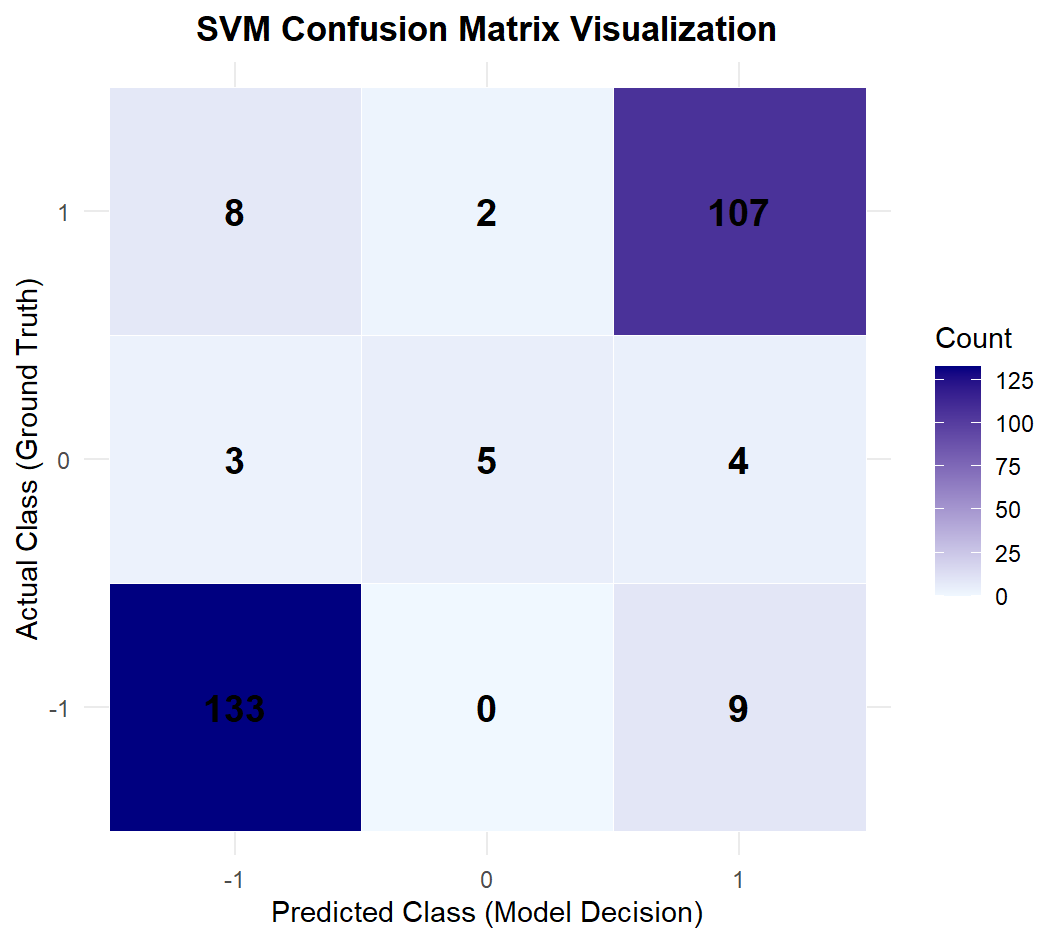
\includegraphics[width=0.65\textwidth]{Rplot02.png} 
		\caption{Heatmap Visualization of the SVM Confusion Matrix.}
		\label{fig:svm_confusion}
	\end{figure}
	
	To provide a comprehensive evaluation of the applied Support Vector Machine method on this website phishing dataset, several critical advantages and disadvantages must be discussed:
	
	\subsection*{Advantages:}
	\begin{itemize}[itemsep=1pt, topsep=2pt]
		\item \textbf{Efficiency with Low Dimensionality:} With exactly 9 input features, SVM efficiently constructs an optimal separating boundary without suffering from high computational complexity.
		\item \textbf{Nonlinear Flexibility:} The Radial Basis Function (RBF) kernel allows the algorithm to effortlessly map complex, nonlinear interactions between technical attributes into a higher-dimensional space where they become separable.
		\item \textbf{Generalisation Capacity:} The soft-margin formulation ($C=1$) prevents overfitting to noise in the training set, allowing the model to remain robust when evaluated on unseen test instances.
	\end{itemize}
	
	\subsection*{Disadvantages:}
	\begin{itemize}[itemsep=1pt, topsep=2pt]
		\item \textbf{Lack of Interpretability:} SVM functions primarily as a ``black box'' model. Unlike decision trees, it does not output straightforward rules, making it difficult to explain to an end-user exactly why a specific URL was flagged.
		\item \textbf{Sensitivity to Hyperparameters:} The classification performance heavily relies on parameters such as $\gamma$ and $C$. Achieving optimal results requires extensive tuning, as poor parameter selection can significantly degrade accuracy.
		\item \textbf{Sensitivity to Class Ambiguity:} The model struggled significantly with the intermediate ``Suspicious (0)'' category, misclassifying a high proportion of those samples due to overlapping geometric characteristics with the other two classes.
	\end{itemize}
	
\end{document}